\documentclass[landscape,footrule]{foils}
\usepackage[lecture-serie]{foiltex-extra}
\usepackage{color}
\usepackage{crysymb}
\usepackage[draft]{crygame}
\usepackage{crypto-ii}
\usepackage{graphics}
\usepackage[pdftex]{graphicx} 


\newcommand{\lecture}{Message Authenitcation}
\newcommand{\lserie}{MTAT.07.003 Cryptology II}
\newcommand{\ldate}{26 March, 2010}
\newcommand{\lauthor}{Sven Laur}
\newcommand{\linst}{University of Tartu}
\graphicspath{{./illustrations/}}


\newcommand{\lastline}{\vspace*{-2ex}}
\newcommand{\spreadappart}{\vspace*{\fill}}




\begin{document}
\titlefoil




\middlefoil{Formal Syntax}



\foilhead[-1.5cm]{Symmetric message authentication}

\centerline{\includegraphics[scale=0.8, angle=-90, clip, trim=1.5cm 1.5cm 14.0cm
  1.5cm]{symmetric-authentication.eps}} 
\vspace*{1ex}
\begin{triangles}
\item A randomised \emph{key generation algorithm} outputs a
  \emph{secret key} $\SK\in\KSPACE$ that must be transferred
  privately to the sender and to the receiver.
\item A \emph{keyed hash function} $\MAC_\SK:\MSPACE\to\TSPACE$ takes
  in a \emph{plaintext} and outputs a corresponding \emph{digest}
  (also known as \emph{hash value} or \emph{tag}).
\item A \emph{verification algorithm}
  $\VERIFY_\SK:\MSPACE\times\CSPACE\to\set{0,1}$ tries to distinguish
  between altered and original message pairs.
\item The authentication primitive is \emph{functional} if for all
  $\SK\gets\GEN$ and $m\in\MSPACE$:
  \centerline{$\VERIFY_\SK(m,\MAC_\SK(m))=1$}
\end{triangles}

\foilhead[-1cm]{Two main attack types}

\textbf{Substitution attacks.}  An adversary substitutes $(m,t)$
  with a different message pair $(\overline{m},\overline{t})$. An
  adversary succeeds in \emph{deception} if
  \begin{align*}
    \VERIFY_\SK(\overline{m},\overline{t})=1
   \qquad\qquad\text{and}\qquad\qquad
    m \neq\overline{m}\enspace.
  \end{align*}
\bigskip

\textbf{Impersonation attacks.}  An adversary tries to create a
  valid message pair $(\overline{m},\overline{t})$ without seeing any
  messages from the sender. An adversary succeeds in
  \emph{deception} if
  \begin{align*}
    \VERIFY_\SK(\overline{m},\overline{t})=1\enspace.
  \end{align*}


\foilhead[-1cm]{Maximal resistance against substitutions}

For clarity, assume that $\MSPACE=\set{0,1}$, $\KSPACE=\set{0,1,2,3}$
and the key is chosen uniformly $\SK\getsu\KSPACE$. Then the keyed
hash function can be viewed as a table.
\begin{center}
  \begin{tabular}{c|c|c|c|c|}
   \multicolumn{1}{c}{  }
   &\multicolumn{1}{c}{0}
   &\multicolumn{1}{c}{1}
   &\multicolumn{1}{c}{2}
   &\multicolumn{1}{c}{3}\\
   \cline{2-5}
    0 & a & b & c & d\\
   \cline{2-5}
    1 & e & f & g & h\\
   \cline{2-5}
  \end{tabular}
\end{center}
\bigskip 

If $a$, $b$, $c$ and $d$ are all different, then the pair $(0,t)$
reveals the key $\SK$ and substitution becomes trivial. Hence, the
optimal layout is following.
\begin{center}
  \begin{tabular}{c|c|c|c|c|}
   \multicolumn{1}{c}{  }
   &\multicolumn{1}{c}{0}
   &\multicolumn{1}{c}{1}
   &\multicolumn{1}{c}{2}
   &\multicolumn{1}{c}{3}\\
   \cline{2-5}
    0 & a & a & b & b\\
   \cline{2-5}
    1 & a & b & a & b\\
   \cline{2-5}
  \end{tabular}
\end{center}




\foilhead[-1cm]{Maximal resistance against impersonation}

Again, assume that $\MSPACE=\set{0,1}$, $\KSPACE=\set{0,1,2,3}$ and
$\SK\getsu\KSPACE$. Then the following keyed hash function achieves
maximal impersonation resistance.
\begin{center}
  \begin{tabular}{c|c|c|c|c|}
   \multicolumn{1}{c}{  }
   &\multicolumn{1}{c}{0}
   &\multicolumn{1}{c}{1}
   &\multicolumn{1}{c}{2}
   &\multicolumn{1}{c}{3}\\
   \cline{2-5}
    0 & a & b & c & d\\
   \cline{2-5}
    1 & a & b & c & d\\
   \cline{2-5}
  \end{tabular}
\end{center}
However, this keyed hash function is insecure against substitution
attacks.\vspace*{1cm}

\textbf{Conclusion.} Security against substitution attacks and
security against impersonation attacks are contradicting requirements.


\middlefoil{Information Theoretical\vspace*{2ex}\\ Security}

\foilhead[-1cm]{Authentication as hypothesis testing}

The procedure $\VERIFY_\SK(\cdot)$ must distinguish between two hypotheses.
\begin{diamonds}
  \item[]$\HYP_0$: The pair $c=(m,t)$ is created by the sender.
  \item[]$\HYP_1$: The pair $c=(\overline{m},\overline{t})$ is created
    by the adversary $\AD$.
\end{diamonds}\vspace*{0ex}
Let $\CCC_0$ and $\CCC_1$ be the corresponding distributions of messages.

Since the ratio of false positives $\pr{\VERIFY_\SK(m,t)=0}$ must be
zero, the optimal verification strategy is the following
 \begin{align*}
   \VERIFY_\SK(c)=1 \quad\Leftrightarrow\quad c\in \supp(\CCC_0)
 \end{align*}
 To defeat the message authentication primitive, the adversary $\AD$
 must chose the distribution $\CCC_1$ such that the ratio of false
 negatives is maximal.

\foilhead[-1cm]{Kullback-Leibler divergence}\enlargethispage{3cm}

Let $(p_x)_{x\in\set{0,1}^*}$ and $(q_x)_{x\in\set{0,1}^*}$ be
probability distributions corresponding to hypotheses $\HYP_0$ and
$\HYP_1$. Then Kullback-Leibler divergence is defined as\vspace*{-1ex}
\begin{align*}
  d(p\|q)\doteq\sum_{x: p_x>0} p_x\cdot  \log_2\frac{p_x}{q_x}\enspace,
\end{align*}\ \vspace*{-3ex}\\
Note that Jensen's inequality assures\vspace*{-1.5ex}
\begin{align*}
  -d(p\|q)&=\sum_{x:p_x>0} p_x\cdot \log_2\frac{q_x}{p_x}\leq
  \log_2 \brak{\sum_{x:p_x>0} q_x}
\end{align*}\ \vspace{-3ex}\\
and consequently\vspace*{-1ex}
\begin{align*}
\sum_{x:p_x>0}q_x\geq 2^{-d(p\|q)}\enspace.
\end{align*}


\foilhead[-1cm]{Lower bound on false positives}

Fix a target message $\overline{m}$. Then by construction
\begin{align*}
  \pr{\VERIFY_\SK(\overline{m},\overline{t})=1}=\sum_{p_{\overline{t},\SK}>0}q_{\overline{t},\SK}\geq
  2^{-d(p\|q)}
\end{align*}
where
\begin{align*}
  p_{\overline{t},\SK}&=\pr{\SK\gets\GEN:\SK\wedge \text{The sender
      creates }
    \overline{t} \text{ for } \overline{m}}\\
  q_{\overline{t},\SK}&=\pr{\SK\gets\GEN:\SK\wedge \text{The adversary
      creates } \overline{t}\text{ for } \overline{m}}
\end{align*}


\foilhead[-1cm]{Simplest impersonation attack}

Consider the following attack
\begin{align*}
  \begin{fblock}{\AD_{\overline{m}}}
    &\overline{\SK}\gets\GEN\\
    &\overline{t}\gets\MAC_{\overline{\SK}}(\overline{m})\\
    &\RETURN (\overline{m},\overline{t})
  \end{fblock}
\end{align*}
Then obviously 
\begin{align*}
  \pr{\,\overline{t}\,}=\sum_{\overline{\SK}}\pr{\SK\gets\GEN:\SK=\overline{\SK}\,}
  \cdot\pr{\overline{t}\gets\MAC_{\overline{\SK}}(\overline{m})}
\end{align*}
is a marginal distribution of $\overline{t}$ generated by the sender.

\foilhead[-1cm]{Success probability}

As $q_{\SK,t}=p_{\SK}\cdot p_t$ the Kullback-Leibler divergence can be further simplified
\begin{align*}
  d(p\|q)&=\sum_{\SK,t}
  p_{t,\SK}\cdot\log_2\frac{p_{t,\SK}}{p_{\SK}\cdot
    p_{t}}\\
 &=\sum_{\SK,t}
  p_{t,\SK}\cdot\log_2 p_{t,\SK}
  -\sum_{\SK,t}
  p_{t,\SK}\log_2 p_{\SK}
  -\sum_{\SK,t}
  p_{t,\SK}\cdot\log_2 p_{t}\\
 &=-H(\SK,t)+H(\SK)+H(t)
\end{align*}
and thus
\begin{align*}
  \pr{\text{Successful impersonation}}\geq
  2^{H(\SK,t)-H(\SK)-H(t)}%
  =2^{-I(\SK:t)}\enspace
\end{align*}
for a fixed target message $\overline{m}$.


\foilhead[-1cm]{An obvious substitution attack}

To replace $m$ with $\overline{m}$, we can use the following strategy:
\begin{align*}
  \begin{fblock}{\AD(m,t,\overline{m})}
    &\SK_*\gets\argmax_{\overline{\SK}}\pr{\SK\gets\GEN: \SK=\overline{\SK}|m,t}\\
    &\overline{t}\gets\MAC_{\SK_*}(\overline{m})\\
    &\RETURN (\overline{m},\overline{t})
  \end{fblock}
\end{align*}
Obviously, the adversary $\AD$ succeeds if it  guesses the key $\SK$
\begin{align*}
  \pr{\mathrm{Success}}&\geq\pr{\SK\gets\GEN:\SK=\SK_*}\\
  &\geq\sum_{t}\pr{t=\MAC_\SK(m)}\cdot\max_{\overline{\SK}}\pr{\SK=\overline{\SK}|t}\enspace.
\end{align*}

\foilhead[-1cm]{Properties of conditional entropy}%\enlargethispage{2cm}

Note that for any distribution $(p_x)_{x\in\set{0,1}^*}$\vspace*{-0.0ex}
\begin{align*}
  H_{\infty}(X)&=-\log_2\brak{\max_{x:p_x>0} p_x}=\min_{x:p_x>0}\brak{-\log_2 p_x}\\
             &\leq \sum_{x:p_x>0} p_x\cdot (-\log_2 p_x)=H(X)\enspace.
\end{align*}\ \vspace*{-2.0ex}\\
Now for two variables\vspace*{-0.0ex}
\begin{align*}
  \sum_{y}\pr{y}\cdot\max_x\pr{x|y}%
  &=\sum_{y} \pr{y}\cdot2^{-H_\infty(X|y)}
  \geq\sum_{y} \pr{y}\cdot2^{-H(X|y)}\\
  &\geq 2^{\sum\limits_y\pr{y}\cdot(-H(X|y))}=2^{-H(X|Y)}\enspace,
\end{align*}
where the second inequality follows from Jensen's inequality.



\foilhead[-1cm]{Lower bound on success probability}

As the success probability of our impersonation attack is 
\begin{align*}
  \pr{\mathrm{Success}}&=\pr{\SK\gets\GEN:\SK=\SK_*}\\
  &=\sum_{t}\pr{t=\MAC_\SK(m)}\cdot\max_{\overline{\SK}}\pr{\SK=\overline{\SK}|t}\enspace,
\end{align*}
we can rewrite in terms of conditional entropy
\begin{align*}
   \pr{\mathrm{Success}}\geq 2^{-H(\SK|t)}\enspace.
\end{align*}

\foilhead[-1cm]{Simmons's lower bounds}

For any message authentication primitive 
\begin{align*}
  \pr{\text{Successful impersonation}}&\geq \max_{m\in\MSPACE} \set{2^{-I(\SK:t)}}\\
  \pr{\text{Successful substitution}}&\geq \max_{m\in\MSPACE} \set{2^{-H(\SK|t)}}
\end{align*}
and thus
\begin{align*}
  \pr{\text{Successful attack}}&\geq \max_{m\in\MSPACE}\set{2^{-\min\set{I(\SK:t),H(\SK|t)}}}
  \geq \max_{m\in\MSPACE}\set{2^{-\frac{H(\SK)}{2}}}
\end{align*}
since $I(\SK:t)=H(\SK)+H(t)-H(\SK,t)=H(\SK)-H(\SK|t)$.

\middlefoil{Examples}

\foilhead[-1cm]{Universal hash functions}

A \emph{universal hash function} $h:\MSPACE\times\KSPACE\to \TSPACE$
is a keyed hash function such that for any two different inputs
$m_0\neq m_1$, the corresponding hash values $h(m_0,k)$ and $h(m_1,k)$
are independent and have a uniform distribution over $\TSPACE$ when
$k$ is chosen uniformly from $\KSPACE$.

\textbf{Corollary.} An authentication protocol that uses a universal
hash function $h$ achieves maximal security against impersonation and
substitution attacks
\begin{align*}
  \pr{\text{Successful deception}}\leq \frac{1}{\abs{\TSPACE}}
\end{align*}

\textbf{Example}. A function $h(m,k_0\|k_1)=k_1\cdot m+k_0$ is a
universal hash function if $\MSPACE=\GF(2^n)$,
$\KSPACE=\GF(2^n)\times\GF(2^n)$ and operations are done
in~$\GF(2^n)$.

\foilhead[-1cm]{Polynomial message authentication code}

Let $m_1,m_2,\ldots,m_\ell$ be $n$-bit blocks of the message and
$k_0,k_1\in\GF(2^n)$ sub-keys for the hash function. Then we can
consider a polynomial
\begin{align*}
  f(x)=m_\ell\cdot x^\ell+m_{\ell-1}\cdot x^{\ell-1}+\cdots+m_1\cdot x 
\end{align*}
over $\GF(2^n)$ and define the hash value as 
\begin{align*}
  h(m,k)=f(k_1)+k_0\enspace.
\end{align*}
If $k_0$ is chosen uniformly over $\GF(2^n)$ then the hash value
$h(m,k)$ is also uniformly distributed over $\GF(2^n)$:
\begin{align*}
  \pr{\text{Successful impersonation}}\leq 2^{-n}\enspace.
\end{align*}

\foilhead[-1cm]{Security against substitution attacks}

Let $\AD$ be the best substitution strategy. W.l.o.g. we can assume
that $\AD$ is a deterministic strategy. Consequently, we have to bound
the  probability
\begin{align*}
  \max_{m\in\MSPACE} \pr{k\gets\KSPACE,
    (\overline{m},\overline{t})\gets
    \AD(m,h(m,k)):h(\overline{m},k)=\overline{t}\wedge m\neq\overline{m}}\enspace.
\end{align*}
Since $\AD$ outputs always the same reply for $k\in\KSPACE$ such that
$h(m,k)=t$, we must find cardinalities of the following sets:
\begin{triangles}
  \item a set of all relevant keys $\KSPACE_{\mathrm{all}}=\set{k\in\KSPACE: h(m,k)=t}$
  \item a set of good keys $\KSPACE_{\mathrm{good}}=\set{k\in\KSPACE:
      h(m,k)=t\wedge h(\overline{m},k)=\overline{t}}$.
\end{triangles}

\foilhead[-1cm]{Some algebraic properties}

For each $m$, $t$ and $k_1$, there exists one and only one value of
$k_0$ such that $h(m,k)=t$. Therefore,
$\abs{\KSPACE_{\mathrm{all}}}=2^{n}$ for any $m$ and $t$.

If $h(m,k)=t$ and $ h(\overline{m},k)=\overline{t}$ then 
\begin{align*}
  h(m,k)-h(\overline{m},k)-t+\overline{t}&=0\\
  \Updownarrow\qquad\qquad&\\
  f_m(k_1)-f_{\overline{m}}(k_1)-t+\overline{t}&=0\\
  \Updownarrow\qquad\qquad&\\
   f_{m-\overline{m}}(k_1)-t+\overline{t}&=0
\end{align*}
This equation has at most $\ell$ solutions $k_1\in\GF(2^n)$, since
degree of $f_{m-\overline{m}}(x)$ is at most $\ell$. Since $k_1$, $m$,
$t$ uniquely determine $k_0$, we get  $\abs{\KSPACE_{\mathrm{good}}}\leq \ell$.

\foilhead[-1cm]{The corresponding bounds}

Hence, we have obtained
\begin{align*}
  \pr{k\gets\KSPACE:h(\overline{m},k)=\overline{t}|m\neq\overline{m},t}
  =\frac{\abs{\KSPACE_{\mathrm{good}}}}{\abs{\KSPACE_{\mathrm{all}}}}\leq\frac{\ell}{2^n}\enspace.
\end{align*}
Since 
\begin{align*}
  & \pr{k\gets\KSPACE,
    (\overline{m},\overline{t})\gets
    \AD(m,h(m,k)):h(\overline{m},k)=\overline{t}\wedge m\neq\overline{m}}\\
  &\leq\sum_{t}\pr{k\gets\KSPACE:h(m,k)=t}\cdot \max_{\overline{m}\neq m\atop \overline{t}\in\TSPACE}
     \pr{h(\overline{m},k)=\overline{t}|m\neq\overline{m},t}\\
  &\leq \sum_{t}\pr{k\gets\KSPACE:h(m,k)=t}\cdot \frac{\ell}{2^n}\leq \frac{\ell}{2^n}\enspace,
\end{align*}
we also have a success bound on substitution attacks. 





\middlefoil{Computational Security}

\foilhead[-1cm]{Authentication with pseudorandom functions}

Consider following authentication primitive:
\begin{triangles}
  \item secret key $f\getsu \FFFALL$ where $\FFFALL=\set{f:\MSPACE\to\TSPACE}$;
  \item authentication code $\MAC_f(m)=f(m)$
  \item verification procedure $\VERIFY_f(m,t)=1\Leftrightarrow f(m)=t$.
\end{triangles}
This authentication primitive is $\frac{1}{\abs{\TSPACE}}$ secure
against impersonation and substitution attacks, since $\MAC$ is a universal hash function. 

As this construction is practically uninstantiable, we must use
$(t,q,\varepsilon)$-pseudorandom function family $\FFF$ instead of
$\FFFALL$. As a result 
\begin{align*}
  \pr{\text{Successful attack}}\leq \frac{1}{\abs{\TSPACE}}+\varepsilon
\end{align*}
against all $t$-time adversaries if $q\geq 1$.  

\foilhead[-1cm]{Formal security definition}

A \emph{keyed hash function} $h:\MSPACE\times\KSPACE\to\TSPACE$ is a
$(t,q,\varepsilon)$-\emph{secure message authentication code} if any $t$-time
adversary $\AD$:
\begin{align*}
  \advMACXX{h}{\AD}=\pr{\GAME^\AD=1}\leq\varepsilon\enspace,
\end{align*}
\ \vspace{-4ex}\\
where the security game is following\vspace*{-1ex}
 \begin{align*}
  \begin{game}{\GAME^\AD}
    &k\getsu\KSPACE\\
    &\!\!\!\begin{forblock}{i\in\set{1,\ldots,q}}
      &\text{Given } m_i\gets \AD \text{ send }
      t_i\gets h(m_i,k) \text{ back to $\AD$}\\
    \end{forblock}\\
    &(m,t)\gets\AD\\
    &\RETURN [t\iseq h(m,k)]\wedge[(m,t)\notin\set{(m_1,t_1),\ldots,(m_q,t_q)}]
  \end{game}
\end{align*}


\foilhead[-1cm]{Problems with multiple sessions}

All authentication primitives we have considered so far guarantee
security if they are used only once. A proper message authentication
protocol can handle many messages. Therefore, we use additional
mechanisms besides the authentication primitive to assure:
\begin{triangles}
  \item security against reflection attacks
  \item message reordering 
  \item interleaving attacks
\end{triangles}
\Bigskip

\textbf{Corresponding enhancement techniques}
\begin{triangles}
  \item Use nonces to defeat reflection attacks.
  \item Use message numbering against reordering.
  \item Stretch secret key using pseudorandom generator.
\end{triangles}

\end{document}